\section{Experiments}

\subsection{Dataset}
\label{sec:dataset}

Our \textit{3DHumanInDesign} dataset consists of $\sim$10k \textit{layered} graphic designs with human images, carefully curated from two sources to ensure diversity and quality. Specifically, we collect 4,479 samples from the \textit{Crello} dataset~\cite{yamaguchi2021canvasvae}, which covers different kinds of graphic designs such as web banners, social media posts and posters.
Additionally, we gather 5,460 magazine covers and posters from \textit{Freepik}\footnote{https://www.freepik.com}.
For the human image on each design, we extract SMPL-H pose parameters and 3D root joint positions (framing parameters) 
using a previous human pose and shape estimation method~\cite{aios}. 
We remove human images from the original designs to create input designs (without human images).
We partition our dataset into training and test splits with a ratio of 8:2, while ensuring that each split has $40 \%$ and $60 \%$ of its samples from Crello and Freepik, respectively.

\subsection{Implementation Details}

For all the three training stages, we optimize our model using AdamW ($\beta_1 = 0.9$, $\beta_2 = 0.95$, weight decay $0.1$) with a base learning rate of $1\times10^{-4}$, using $1{,}000$ warm-up iterations followed by a cosine decay schedule. We use a batch size of $16$, a gradient-norm clip of $1.0$, a label smoothing of $0.05$, and maintain an exponential moving average of the weights with a decay of $0.995$.At inference time, We employ top-$p$ sampling with temperature $0.8$ and $p = 0.8$.

\subsection{Baselines}

Since there is no prior work on design-conditioned 3D human adding, we compare our method against two baselines:

\begin{itemize}
    \item \textit{FlexDM}. FlexDM~\cite{flexdm} is a unified model for solving different design tasks.
    We fine-tune FlexDM on our training set, 
    and adapt it to our problem by empolying a two-stage approach. In the first stage, we utilize FlexDM to solve an image filling task to produce an image embedding, by feeding all the elements in the input design, along with an added image element (with all the fields masked out except its category), into FlexDM. The output image embedding is used to retrieve an existing image from a database of realistic human images (taken from the designs in the test set) 
    via cosine similarity between image embeddings. Then, the pose and framing parameters are estimated from the retrieve image using an off-the-shelf human pose and shape estimation method~\cite{aios}.
    In the second stage, we use FlexDM to perform layout generation for the retrieved image.
    Since FlexDM can not predict the z-order of an element, for a fair comparison, we use the z-order generated by our model when composing the human image into the input design. 

    \item \textit{MLLM.} We design a baseline leveraging multimodal large language models (MLLM) for 
    design-conditioned 3D human adding.
    Specifically, we provide the input design image along with its layout information (in textual format) to Gemini 3 Pro~\cite{geminiteam2023gemini}, and prompt it to predict: 1) a text description for a human image; 2) the bounding box parameters and z-order of the human image in the design. The image description is then fed into a text-to-image model, Nano Banana Pro~\cite{google2025nanobanana}, to generate a realistic human image.
    Finally, the pose and framing parameters are extracted from the generated image using an off-the-shelf human pose and shape estimation method~\cite{aios}.
\end{itemize}

\subsection{Evaluation Metrics}
We quantitatively evaluate the performance of our method using four metrics that cover complementary aspects: human-design coherence, overall design quality, pose accuracy, and layout quality.

\begin{itemize}
    \item \textit{Human-Design Alignment (HD-Align).} Inspired by CLIP~\cite{clip}, we train a contrastive model to learn a joint embedding space of human representations and partial designs (with human images excluded), where matched human and design lie close and unmatched ones fall far apart. 
    Our human representation combines the 3D pose, framing, and human image layout information.
    We compute cosine similarity between human and design embeddings as a HD-Align score, with higher HD-Align indicating better human-design coherence.
    \item \textit{Design FID (D-FID).} We train a variational autoencoder that encodes both a human representation (combining 3D pose, framing, and human image layout information) and a partial design (without any human image) into a holistic design embedding. We use these embeddings to compute Fr\'{e}chet Inception Distance (FID) between generated and real designs as a measure of overall design quality. Lower D-FID indicates better holistic design quality.
    \item \textit{MPJPE.} We adopt Mean Per Joint Position Error (MPJPE), a common metric for 3D human pose estimation, 
    to evaluate predicted 3D poses,
    which computes the mean Euclidean distance between predicted and ground-truth 3D joint positions.
    \item \textit{Alignment, Overlap.} We evaluate the quality of predicted human image layouts (bounding boxes) with two widely used metrics in the layout generation literature, \textit{Alignment} and \textit{Overlap}~\cite{LayoutGAN}. Both metrics are computed on the layouts of complete designs with human images included. 
\end{itemize}

\subsection{Quantitative Results}

\begin{table}[t]
\centering
\caption{Quantitative evaluation results of different methods. The best results are in bold, while the second best results are underlined.}
\label{tab:quantitative_results}
\resizebox{\columnwidth}{!}{%
\begin{tabular}{l|ccccc}
\hline
Method
& HD-Align~$\uparrow$ & D-FID~$\downarrow$  
& MPJPE~$\downarrow$ 
& Align~$\downarrow$ & Overlap~$\downarrow$ \\
\hline
FlexDM     & 4.65 & \underline{3.90}& \underline{2176.29} & \underline{0.17} & 213.39 \\
MLLM       & \underline{5.26} & 7.95 & 2829.97 & 0.20 & \textbf{196.03} \\
Ours       & \textbf{6.52} & \textbf{0.07} & \textbf{385.12} & \textbf{0.17} & \underline{209.11} \\
\hline
Real Data  & 7.06 & -- & -- & 0.16 & 210.48 \\
\hline
\end{tabular}%
}
\end{table}

Table~\ref{tab:quantitative_results} reports the quantitative results of different methods on the test set. The HD-Align score of our method is better than those of the baselines by significant margins, while being competitive with that of the read data (samples in the test set). 
This suggest great alignment of our generated human pose, framing and human image layout with the design context. Our method also shows a noticeable improvement in D-FID compared to the other methods, highlighting the superior quality of holistic designs (with added human images) generated by our method. Our method significantly outperforms the baselines in MPJPE, confirming that its generated poses are closer to the ground truth. In addition, our method achieves the best alignment score and the second best overlap score, which means that our method can result in spatially cohesive design layouts after adding human images into the partial designs. Although MLLM yields the lowest overlap score, the overlap score of our method (209.11) is quite close to that of the real data (210.48), which suggests that our resulting layouts encompass a similar amount of overlap between elements to real designs.   

\begin{figure*}[t]
  \centering
  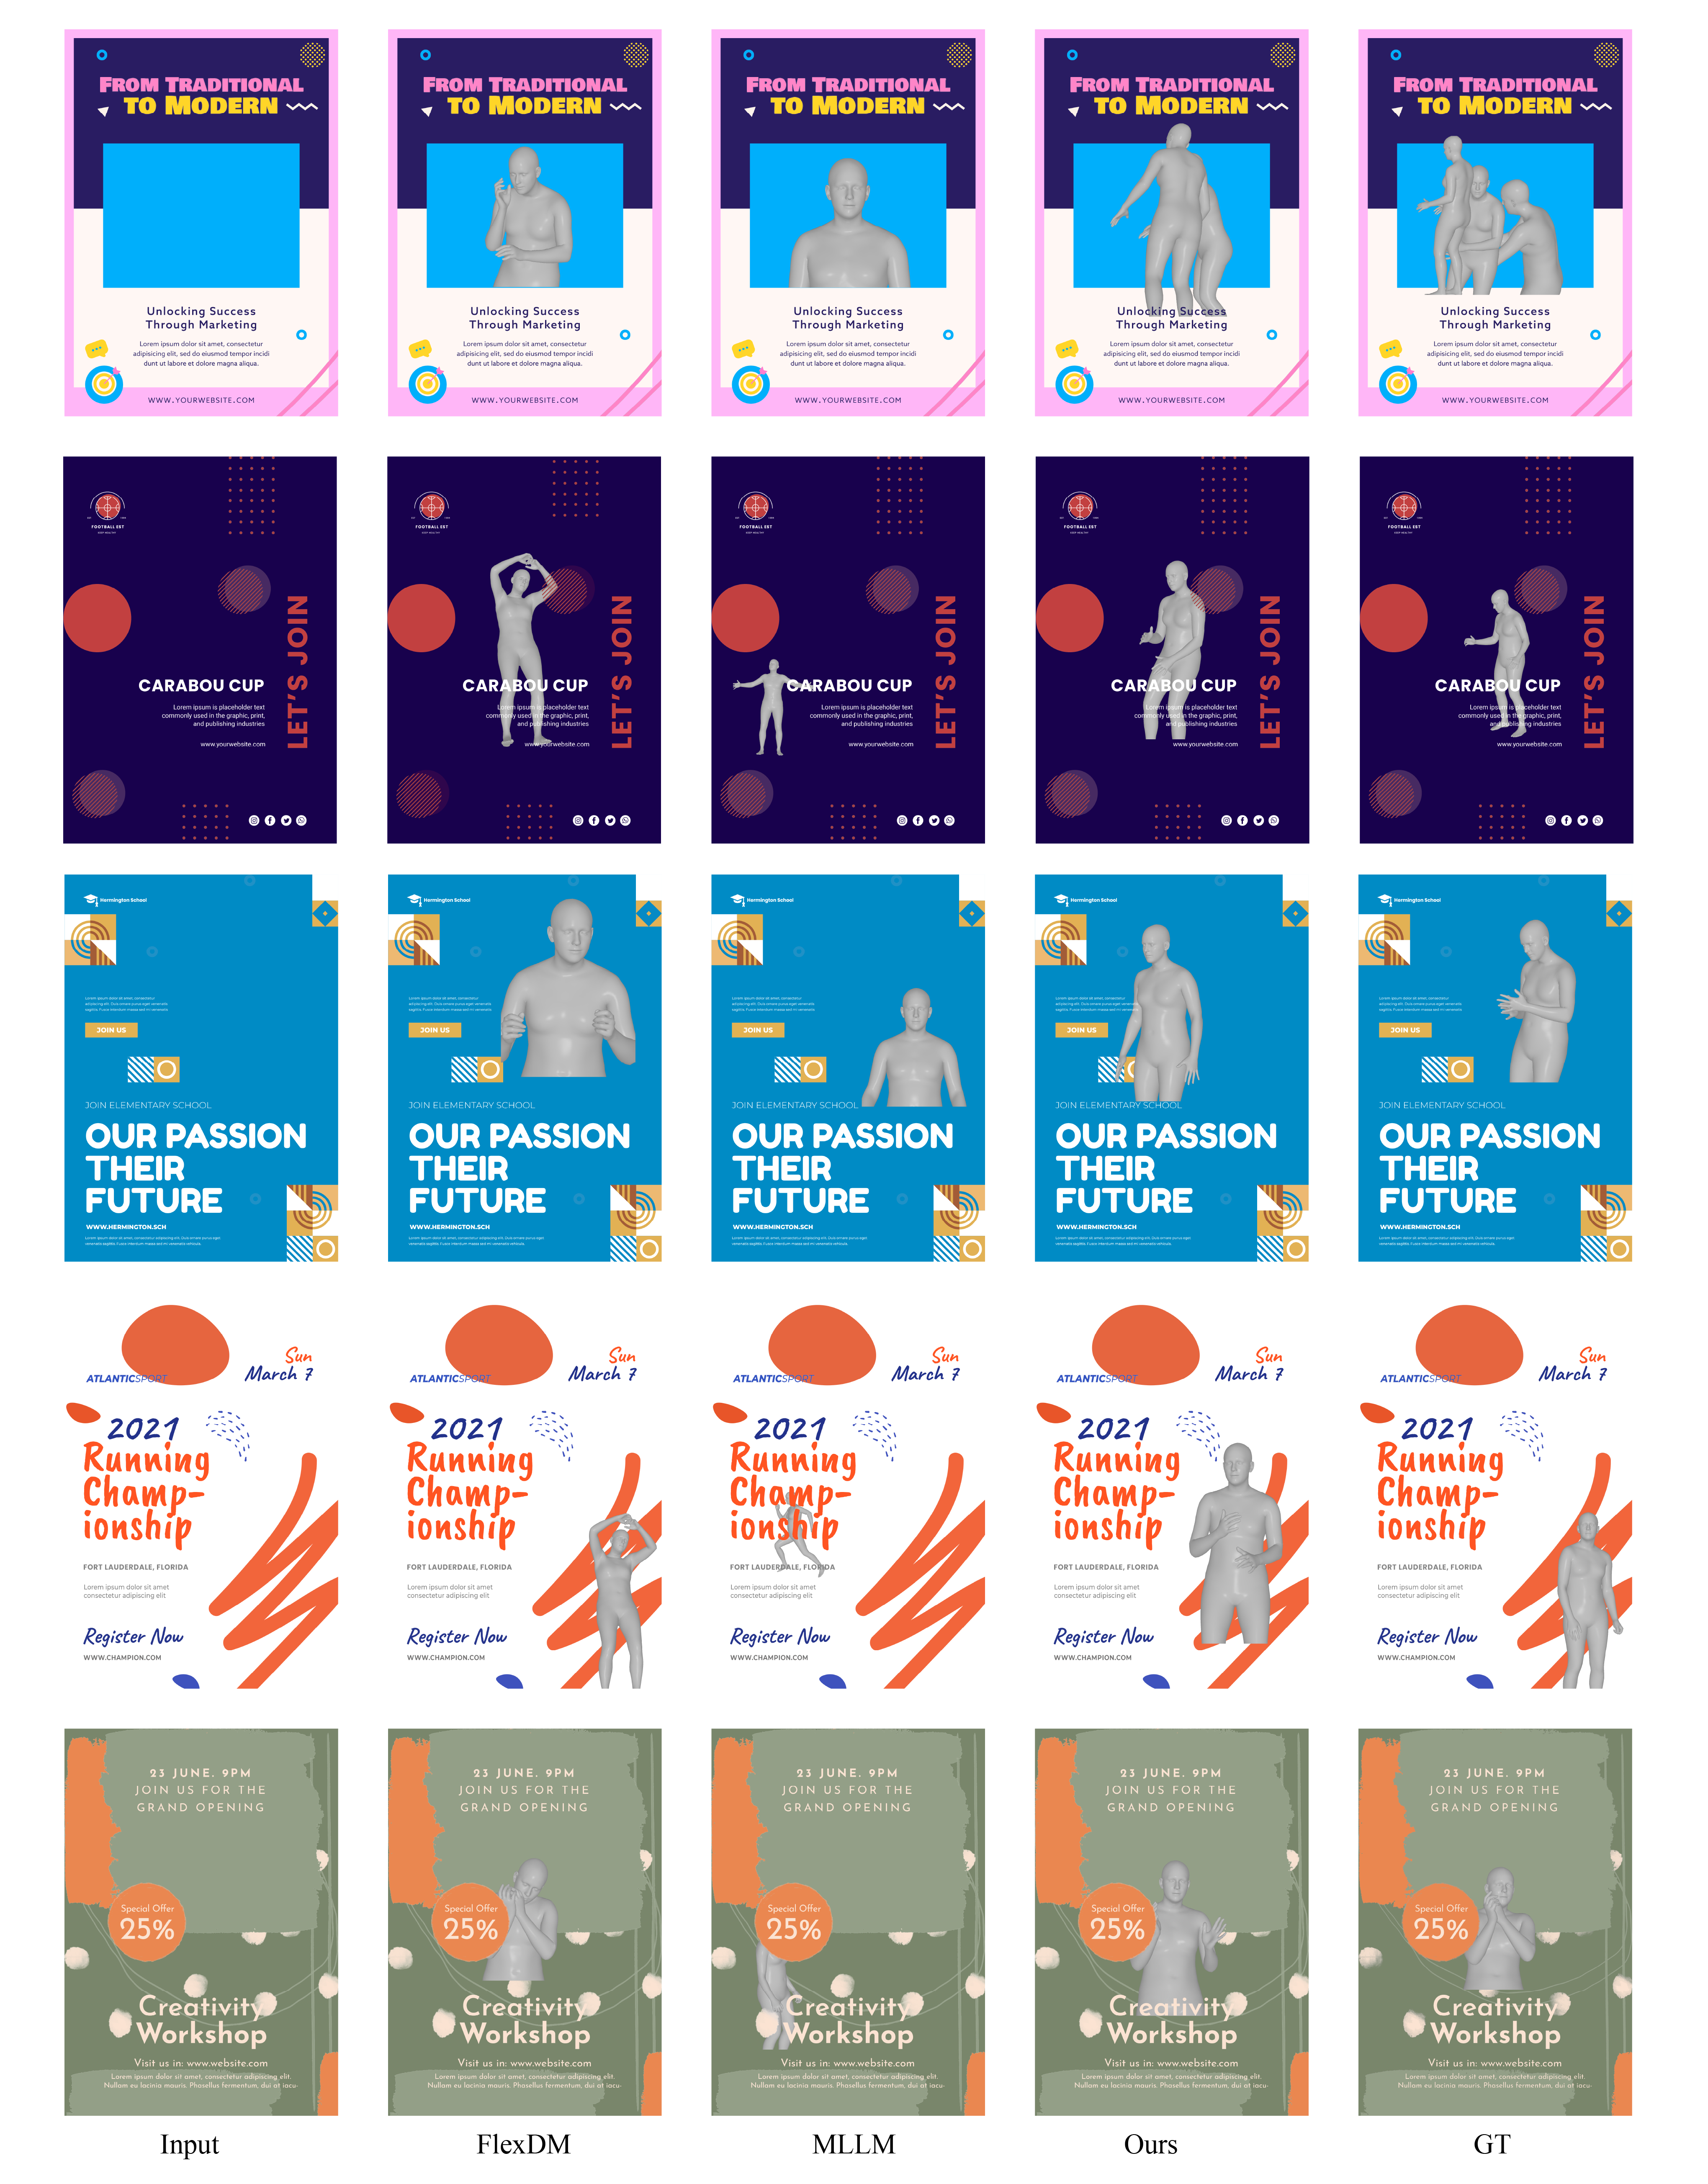
\includegraphics[width=0.9\linewidth]{figure/fig4_comparison.png}
  \caption{
  Qualitative comparison of different methods.
  }
  \label{fig:comparison}
\end{figure*}

\begin{figure*}[t]
  \centering
  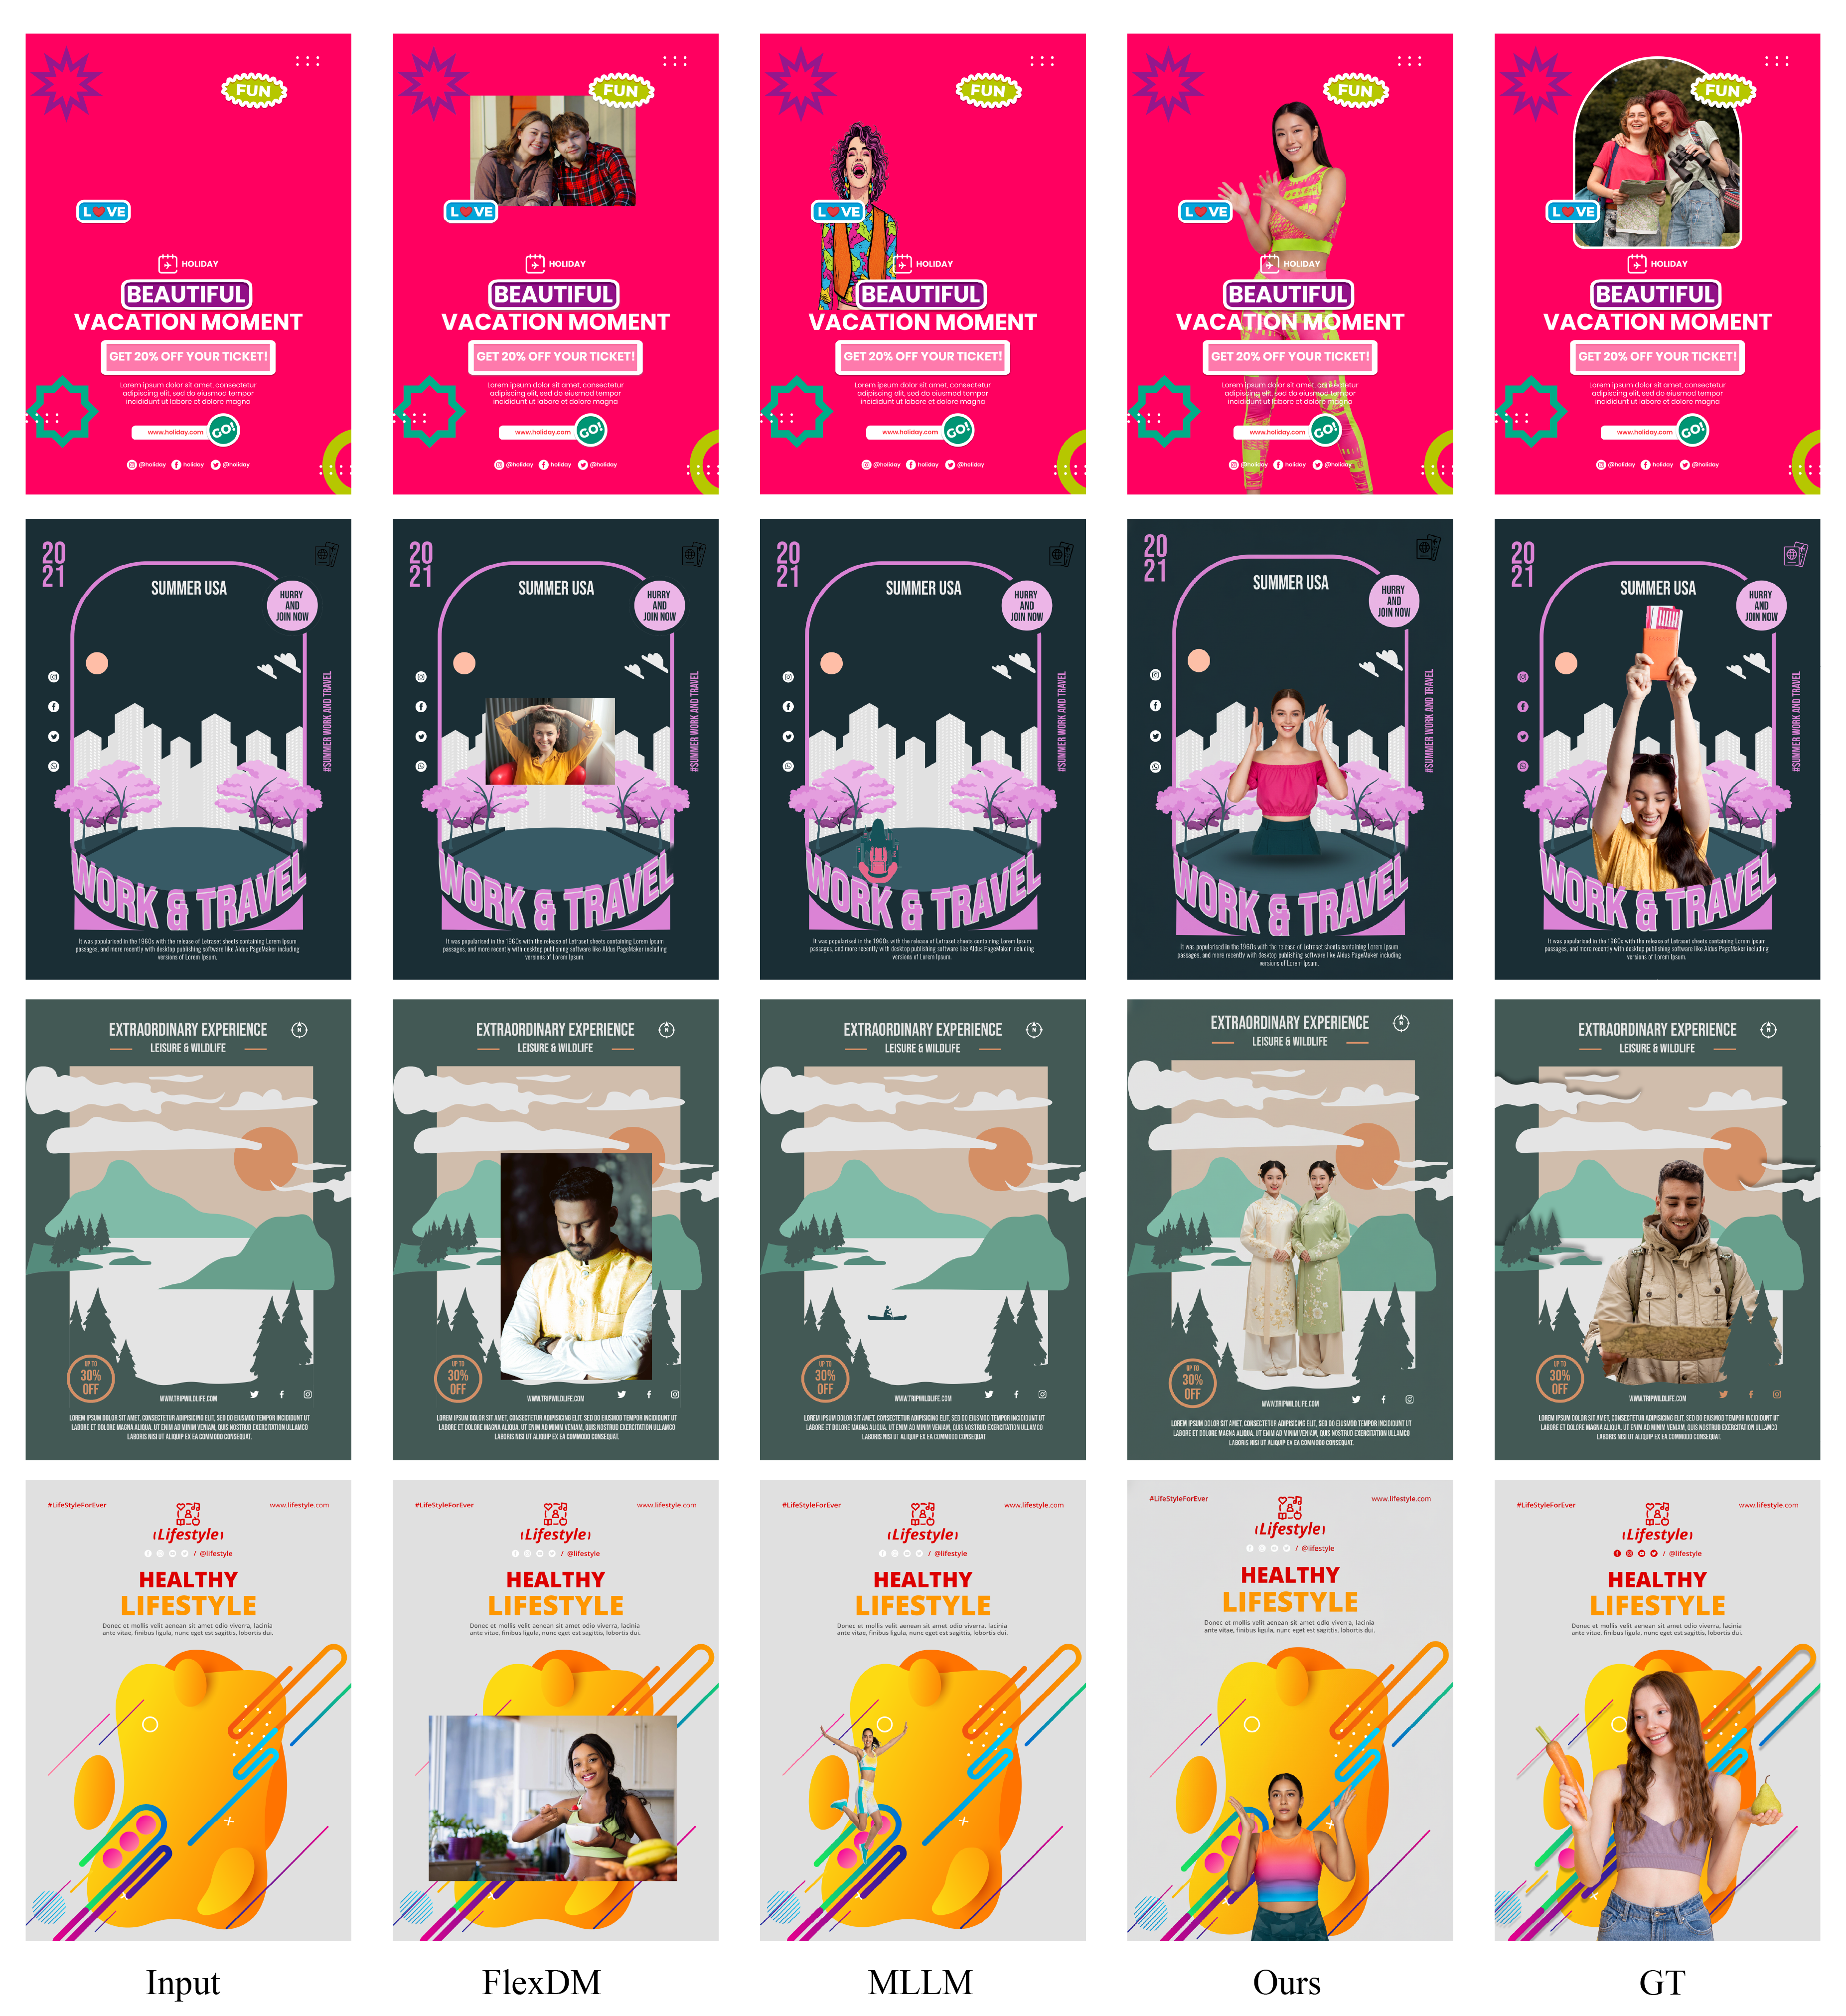
\includegraphics[width=0.85\linewidth]{figure/fig5_rendering.png}
  \caption{Results of different methods where realistic human images are added.
  }
  \label{fig:rendering}
\end{figure*}

\subsection{Qualitative Results}

Figure~\ref{fig:comparison} shows visual comparison of results from different methods. As compared with the baselines, our method can generate 3D human poses and 2D framing that better harmonizes with the design context and more closely resemble what professional designers create. For example, in the first row, our method add multiple humans whose \textit{body orientations} are similar to those of humans in the ground truth design, whereas FlexDM and MLLM generates a single human facing outwards. In the third row, our method frames the added human in the same way as the real design\textemdash a \textit{medium full shot} is used, capturing the human from the top of the head to just below the waist, while FlexDM and MLLM employ a \textit{medium shot} that starts just above the head and ends around the waist. In addition, our method is able to generate human image layouts that are spatially compatible with the remaining design elements. MLLM sometimes falls shot of predicting proper bounding box coordinates and z-order for the added human image, causing visual conflict between the human image and other design elements; for example, a large portion of the added human is occluded by the texts in the fourth row.
    

\subsection{User Study}

\begin{table}[t]
\centering
\caption{User study results. For each aspect, the percentage of the time that each method is chosen as the best is reported.
}
\label{tab:user_study}
\resizebox{0.85\columnwidth}{!}
{
\begin{tabular}{l|cc}
\hline
 Method & Human-Design Align & Aesthetic Quality\\
\hline
FlexDM  & 11.9\% & 17.8\% \\
MLLM &  27.0\% & 22.5\% \\
Ours & \textbf{61.1\%} & \textbf{59.7\%} \\
\hline
\end{tabular}
}
\end{table}

We conduct a user study comparing our method with FlexDM and MLLM for \textit{human-design alignment} and \textit{aesthetic quality}. We apply each method to 100 input designs from our test set to generate complete designs (with realistic human images added). Our study involves 23 professional graphic designers. The participants are shown three generated complete designs by different methods in randomized order, along with the input design and ground truth design for reference, and asked to evaluate the generated designs in terms of two aspects: 1) human-design alignment (whether the added human image fits well the remaining part of the design in terms of human pose, framing and image layout; 2) aesthetic quality (whether the design looks visually aesthetic). For each aspect, the participants are asked to choose the best generated design. The results are shown in Table ~\ref{tab:user_study}. Our method is significantly preferred over the other methods on both aspects, suggesting that our method is able to achieve better human-design alignment and aesthetic quality. Figure \ref{fig:rendering} shows some results of different methods that are displayed in the user study.